% Options for packages loaded elsewhere
\PassOptionsToPackage{unicode}{hyperref}
\PassOptionsToPackage{hyphens}{url}
%
\documentclass[
  man,floatsintext]{apa6}
\usepackage{amsmath,amssymb}
\usepackage{iftex}
\ifPDFTeX
  \usepackage[T1]{fontenc}
  \usepackage[utf8]{inputenc}
  \usepackage{textcomp} % provide euro and other symbols
\else % if luatex or xetex
  \usepackage{unicode-math} % this also loads fontspec
  \defaultfontfeatures{Scale=MatchLowercase}
  \defaultfontfeatures[\rmfamily]{Ligatures=TeX,Scale=1}
\fi
\usepackage{lmodern}
\ifPDFTeX\else
  % xetex/luatex font selection
\fi
% Use upquote if available, for straight quotes in verbatim environments
\IfFileExists{upquote.sty}{\usepackage{upquote}}{}
\IfFileExists{microtype.sty}{% use microtype if available
  \usepackage[]{microtype}
  \UseMicrotypeSet[protrusion]{basicmath} % disable protrusion for tt fonts
}{}
\makeatletter
\@ifundefined{KOMAClassName}{% if non-KOMA class
  \IfFileExists{parskip.sty}{%
    \usepackage{parskip}
  }{% else
    \setlength{\parindent}{0pt}
    \setlength{\parskip}{6pt plus 2pt minus 1pt}}
}{% if KOMA class
  \KOMAoptions{parskip=half}}
\makeatother
\usepackage{xcolor}
\usepackage{graphicx}
\makeatletter
\def\maxwidth{\ifdim\Gin@nat@width>\linewidth\linewidth\else\Gin@nat@width\fi}
\def\maxheight{\ifdim\Gin@nat@height>\textheight\textheight\else\Gin@nat@height\fi}
\makeatother
% Scale images if necessary, so that they will not overflow the page
% margins by default, and it is still possible to overwrite the defaults
% using explicit options in \includegraphics[width, height, ...]{}
\setkeys{Gin}{width=\maxwidth,height=\maxheight,keepaspectratio}
% Set default figure placement to htbp
\makeatletter
\def\fps@figure{htbp}
\makeatother
\setlength{\emergencystretch}{3em} % prevent overfull lines
\providecommand{\tightlist}{%
  \setlength{\itemsep}{0pt}\setlength{\parskip}{0pt}}
\setcounter{secnumdepth}{-\maxdimen} % remove section numbering
% Make \paragraph and \subparagraph free-standing
\makeatletter
\ifx\paragraph\undefined\else
  \let\oldparagraph\paragraph
  \renewcommand{\paragraph}{
    \@ifstar
      \xxxParagraphStar
      \xxxParagraphNoStar
  }
  \newcommand{\xxxParagraphStar}[1]{\oldparagraph*{#1}\mbox{}}
  \newcommand{\xxxParagraphNoStar}[1]{\oldparagraph{#1}\mbox{}}
\fi
\ifx\subparagraph\undefined\else
  \let\oldsubparagraph\subparagraph
  \renewcommand{\subparagraph}{
    \@ifstar
      \xxxSubParagraphStar
      \xxxSubParagraphNoStar
  }
  \newcommand{\xxxSubParagraphStar}[1]{\oldsubparagraph*{#1}\mbox{}}
  \newcommand{\xxxSubParagraphNoStar}[1]{\oldsubparagraph{#1}\mbox{}}
\fi
\makeatother
% definitions for citeproc citations
\NewDocumentCommand\citeproctext{}{}
\NewDocumentCommand\citeproc{mm}{%
  \begingroup\def\citeproctext{#2}\cite{#1}\endgroup}
\makeatletter
 % allow citations to break across lines
 \let\@cite@ofmt\@firstofone
 % avoid brackets around text for \cite:
 \def\@biblabel#1{}
 \def\@cite#1#2{{#1\if@tempswa , #2\fi}}
\makeatother
\newlength{\cslhangindent}
\setlength{\cslhangindent}{1.5em}
\newlength{\csllabelwidth}
\setlength{\csllabelwidth}{3em}
\newenvironment{CSLReferences}[2] % #1 hanging-indent, #2 entry-spacing
 {\begin{list}{}{%
  \setlength{\itemindent}{0pt}
  \setlength{\leftmargin}{0pt}
  \setlength{\parsep}{0pt}
  % turn on hanging indent if param 1 is 1
  \ifodd #1
   \setlength{\leftmargin}{\cslhangindent}
   \setlength{\itemindent}{-1\cslhangindent}
  \fi
  % set entry spacing
  \setlength{\itemsep}{#2\baselineskip}}}
 {\end{list}}
\usepackage{calc}
\newcommand{\CSLBlock}[1]{\hfill\break\parbox[t]{\linewidth}{\strut\ignorespaces#1\strut}}
\newcommand{\CSLLeftMargin}[1]{\parbox[t]{\csllabelwidth}{\strut#1\strut}}
\newcommand{\CSLRightInline}[1]{\parbox[t]{\linewidth - \csllabelwidth}{\strut#1\strut}}
\newcommand{\CSLIndent}[1]{\hspace{\cslhangindent}#1}
\ifLuaTeX
\usepackage[bidi=basic]{babel}
\else
\usepackage[bidi=default]{babel}
\fi
\babelprovide[main,import]{english}
% get rid of language-specific shorthands (see #6817):
\let\LanguageShortHands\languageshorthands
\def\languageshorthands#1{}
% Manuscript styling
\usepackage{upgreek}
\captionsetup{font=singlespacing,justification=justified}

% Table formatting
\usepackage{longtable}
\usepackage{lscape}
% \usepackage[counterclockwise]{rotating}   % Landscape page setup for large tables
\usepackage{multirow}		% Table styling
\usepackage{tabularx}		% Control Column width
\usepackage[flushleft]{threeparttable}	% Allows for three part tables with a specified notes section
\usepackage{threeparttablex}            % Lets threeparttable work with longtable

% Create new environments so endfloat can handle them
% \newenvironment{ltable}
%   {\begin{landscape}\centering\begin{threeparttable}}
%   {\end{threeparttable}\end{landscape}}
\newenvironment{lltable}{\begin{landscape}\centering\begin{ThreePartTable}}{\end{ThreePartTable}\end{landscape}}

% Enables adjusting longtable caption width to table width
% Solution found at http://golatex.de/longtable-mit-caption-so-breit-wie-die-tabelle-t15767.html
\makeatletter
\newcommand\LastLTentrywidth{1em}
\newlength\longtablewidth
\setlength{\longtablewidth}{1in}
\newcommand{\getlongtablewidth}{\begingroup \ifcsname LT@\roman{LT@tables}\endcsname \global\longtablewidth=0pt \renewcommand{\LT@entry}[2]{\global\advance\longtablewidth by ##2\relax\gdef\LastLTentrywidth{##2}}\@nameuse{LT@\roman{LT@tables}} \fi \endgroup}

% \setlength{\parindent}{0.5in}
% \setlength{\parskip}{0pt plus 0pt minus 0pt}

% Overwrite redefinition of paragraph and subparagraph by the default LaTeX template
% See https://github.com/crsh/papaja/issues/292
\makeatletter
\renewcommand{\paragraph}{\@startsection{paragraph}{4}{\parindent}%
  {0\baselineskip \@plus 0.2ex \@minus 0.2ex}%
  {-1em}%
  {\normalfont\normalsize\bfseries\itshape\typesectitle}}

\renewcommand{\subparagraph}[1]{\@startsection{subparagraph}{5}{1em}%
  {0\baselineskip \@plus 0.2ex \@minus 0.2ex}%
  {-\z@\relax}%
  {\normalfont\normalsize\itshape\hspace{\parindent}{#1}\textit{\addperi}}{\relax}}
\makeatother

\makeatletter
\usepackage{etoolbox}
\patchcmd{\maketitle}
  {\section{\normalfont\normalsize\abstractname}}
  {\section*{\normalfont\normalsize\abstractname}}
  {}{\typeout{Failed to patch abstract.}}
\patchcmd{\maketitle}
  {\section{\protect\normalfont{\@title}}}
  {\section*{\protect\normalfont{\@title}}}
  {}{\typeout{Failed to patch title.}}
\makeatother

\usepackage{xpatch}
\makeatletter
\xapptocmd\appendix
  {\xapptocmd\section
    {\addcontentsline{toc}{section}{\appendixname\ifoneappendix\else~\theappendix\fi: #1}}
    {}{\InnerPatchFailed}%
  }
{}{\PatchFailed}
\makeatother
\usepackage{csquotes}
\ifLuaTeX
  \usepackage{selnolig}  % disable illegal ligatures
\fi
\usepackage{bookmark}
\IfFileExists{xurl.sty}{\usepackage{xurl}}{} % add URL line breaks if available
\urlstyle{same}
\hypersetup{
  pdftitle={ChildLens: An Egocentric Video Dataset for Activity Analysis in Children},
  pdfauthor={Nele-Pauline Suffo1, Pierre-Etienne Martin2, Daniel Haun2, \& Manuel Bohn1, 2},
  pdflang={en-EN},
  hidelinks,
  pdfcreator={LaTeX via pandoc}}

\title{ChildLens: An Egocentric Video Dataset for Activity Analysis in Children}
\author{Nele-Pauline Suffo\textsuperscript{1}, Pierre-Etienne Martin\textsuperscript{2}, Daniel Haun\textsuperscript{2}, \& Manuel Bohn\textsuperscript{1, 2}}
\date{}


\shorttitle{ChildLens Dataset}

\authornote{

The authors made the following contributions. Nele-Pauline Suffo: Conceptualization, Writing - Original Draft Preparation, Writing - Review \& Editing; Manuel Bohn: Writing - Review \& Editing, Supervision.

Correspondence concerning this article should be addressed to Nele-Pauline Suffo, Universitätsallee 1, 21335 Lüneburg. E-mail: \href{mailto:nele.suffo@leuphana.de}{\nolinkurl{nele.suffo@leuphana.de}}

}

\affiliation{\vspace{0.5cm}\textsuperscript{1} Institute of Psychology in Education, Leuphana University Lüneburg\\\textsuperscript{2} Max Planck Institute for Evolutionary Anthropology}

\abstract{%
We present ChildLens, a novel egocentric video and audio dataset of children aged 3--5 years, featuring detailed activity labels. Spanning 106 hours of recordings, the dataset includes five location classes and 14 activity classes, covering audio-only, video-only, and multimodal activities. Captured through a vest equipped with an embedded camera, ChildLens provides a rich resource for analyzing children's daily interactions and behaviors. We provide an overview of the dataset, the collection process, and the labeling strategy. Additionally, we present benchmark performance of two state-of-the-art models on the dataset: the Boundary-Matching Network for Temporal Activity Localization and the Voice-Type Classifier for detecting speech in audio. Finally, we analyze the dataset specifications and their influence on model performance. The ChildLens dataset will be made available for research purposes, providing rich data to advance computer vision and audio analysis techniques while offering new insights into developmental psychology.
}



\begin{document}
\maketitle

\section{Introduction}\label{introduction}

In developmental psychology, children's everyday experiences are widely recognized as crucial for shaping their cognitive, emotional, and social development (Rogoff, Dahl, \& Callanan, 2018). For instance, Spangler (1989) shows that toddlers' daily interactions influence their mental and emotional dispositions and predict later mental and motivational development. Additionally, De Barbaro and Fausey (2022) emphasize the dynamic and diverse nature of infants' experiences as captured by everyday activity sensors, highlighting the need to analyze these interactions over extended periods to fully understand their patterns, variability, and developmental significance. Despite the recognized importance of these experiences, research directly examining their developmental implications remains limited.

Recent studies exploring children's perspectives and their perception of the surrounding environment have often focused exclusively on either the audio component of the data (Roy, Frank, DeCamp, Miller, \& Roy, 2015; Sullivan, Mei, Perfors, Wojcik, \& Frank, 2021), the video data alone (Borjon et al., 2018; Saber, Hansaria, Wood, Smith, \& Tiganj, 2023; Smith, Yu, Yoshida, \& Fausey, 2015; Yoshida \& Smith, 2008), or concentrated on infants under the age of two years (Sullivan et al., 2021; Tsutsui, Chandrasekaran, Reza, Crandall, \& Yu, 2020). However, combining audio and video data in a multimodal dataset offers a more comprehensive understanding of children's activities and interactions. While this approach has been used in studies of adults (Kapidis, Poppe, Van Dam, Noldus, \& Veltkamp, 2020; Truong \& Luu, 2024), it is still not widely explored for children. For instance, Long et al. (2024) introduced the BabyView dataset, a large-scale multimodal dataset capturing egocentric experiences of children aged 6 months to 5 years. While it supports tasks like speech transcription and pose estimation, it does not address activity localization, leaving a key gap in understanding children's daily interactions.

To address this gap, we introduce the ChildLens dataset, a novel egocentric multimodal dataset documenting the everyday experiences of children aged 3--5 years, with a particular focus on detailed activity labels. The dataset consists of 106 hours of video and audio recordings collected from 61 children wearing camera-equipped vests. It includes annotations for five location classes and 14 activity classes, spanning audio-only, video-only, and multimodal activities. Each activity is labeled with its start and end times, activity class, and whether the child is interacting alone or with others. Designed to support research in developmental psychology and computer vision, the ChildLens dataset provides a rich resource for studying children's daily activities and advancing multimodal learning.

\section{Dataset Overview}\label{dataset-overview}

\paragraph{Activity Classes}\label{activity-classes}

The ChildLens dataset contains a total of 14 activity and 5 location classes. The activities are based on the activities of the child in the video and can be divided into \emph{person-only} activities, such as ``child talking'' or ``other person talking'', and \emph{person-object} activities, such as ``drawing'' or ``playing with object''. You can find a brief description of each class in the appendix. The activities can be further divided into \emph{audio-based}, \emph{visual-based}, and \emph{multimodal} activities, as presented in figure \ref{fig:camera-superannotate-activity-classes}. The following list provides an overview of the different activity types:

\begin{itemize}
\tightlist
\item
  \textbf{Audio-based activities}: \emph{child talking}, \emph{other person talking}, \emph{overheard speech}, \emph{singing / humming}, \emph{listening to music / audiobook}
\item
  \textbf{Visual-based activities}: \emph{watching something}, \emph{drawing}, \emph{crafting things}, \emph{dancing}
\item
  \textbf{Multimodal activities}: \emph{playing with object}, \emph{playing without object}, \emph{making music}, \emph{pretend play}, \emph{reading book},
\end{itemize}

The location classes describe the current location of the child in the video and include \emph{livingroom}, \emph{playroom}, \emph{bathroom}, \emph{hallway}, and \emph{other}.

\begin{figure}

{\centering 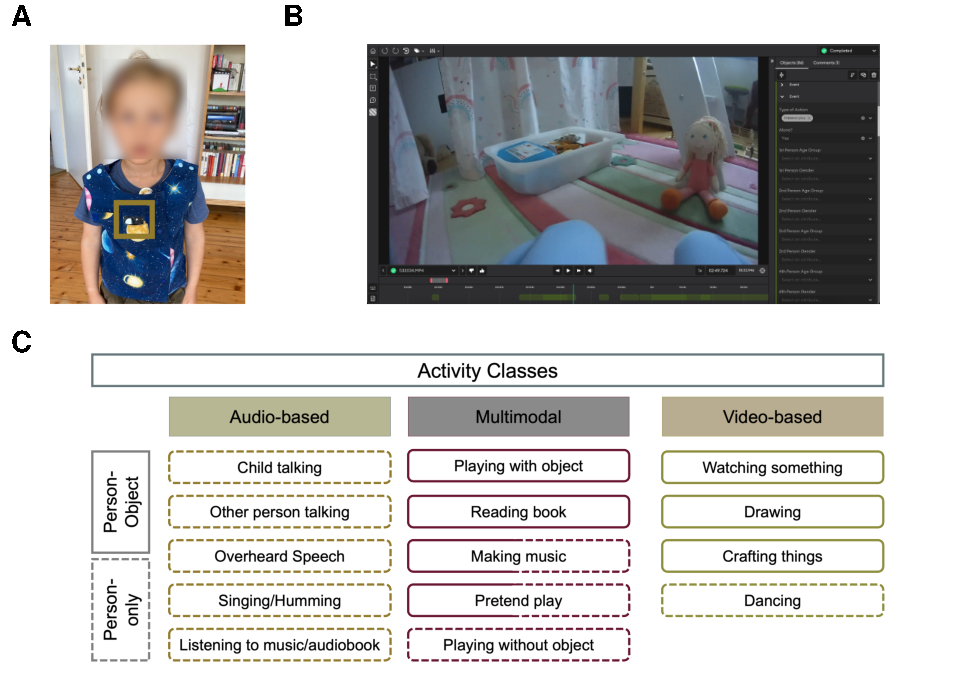
\includegraphics{ChildLens_paper_files/figure-latex/camera-superannotate-activity-classes-1} 

}

\caption{\textbf{A} – Vest with the embedded camera worn by the children, \textbf{B} – SuperAnnotate platform utilized for video annotation, \textbf{C} – Activity classes in the ChildLens dataset.}\label{fig:camera-superannotate-activity-classes}
\end{figure}

\paragraph{Statistics}\label{statistics}

The ChildLens dataset comprises of 343 video files with a total of 106.10 hours recorded by 61 children aged 3 to 5 years (M=4.52, SD=0.92). It includes 107 videos from children aged 3, 122 videos from children aged 4, and 114 videos from children aged 5. The duration of recorded video material per child varies between 4.03 and 303.42 minutes (M=104.37, SD=51.65). A detailed distribution of the video duration per child can be found in figure \ref{fig:minutes-per-child}.

This diverse dataset includes a varying number of instances across the 14 activity classes, ranging from \textbf{x} to \textbf{x} instances per class. The duration of each instance varies by activity. For example, audio-based activities like ``child talking'' may last only a few seconds, while activities like ``reading a book'' can span several minutes. The table with the total number of instances and summed duration for all activity classes is available in the appendix.

\begin{figure}
\centering
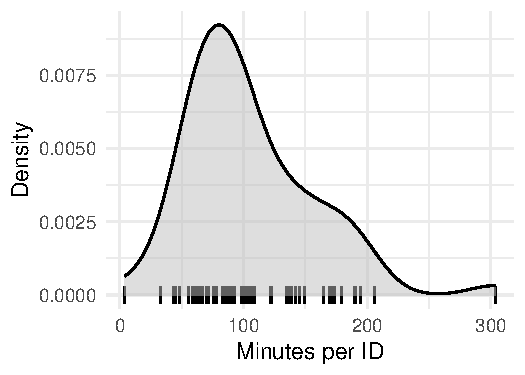
\includegraphics{ChildLens_paper_files/figure-latex/minutes-per-child-1.pdf}
\caption{\label{fig:minutes-per-child}Video recording duration (in minutes) per child ID.}
\end{figure}

\paragraph{Exhaustive multi-label annotations}\label{exhaustive-multi-label-annotations}

The dataset provides detailed annotations for each video file. These annotations specify the child's current location within the video, the start and end times of each activity, the activity class, and whether the child is engaged alone or with somebody else. For every person involved in the activity, we capture age and gender. If multiple activities occur simultaneously in a video, each activity is individually labeled and extracted as a separate clip. For example, if a segment shows a child ``reading a book'' while also ``talking,'' two separate clips are created: one for ``reading a book'' and another for ``child talking.'' This exhaustive labeling strategy ensures that each activity is accurately represented in the dataset.

\section{Dataset Generation}\label{dataset-generation}

This section outlines the steps taken to create the ChildLens dataset. We provide detailed information on the video collection process, the labeling strategy employed, and the generation of activity labels.

\subsection{Step 1: Collection of Egocentric Videos}\label{step-1-collection-of-egocentric-videos}

The ChildLens dataset consists of egocentric videos recorded by children aged 3 to 5 years over a period of 12 months. A total of 61 children from families living in a mid-sized city in Germany, participated in the study. The videos were captured at home using a camera embedded in a vest worn by the children, which can be seen in figure \ref{fig:camera-superannotate-activity-classes}. This setup allowed the children to move freely throughout their homes while recording their activities. The camera, a \emph{PatrolEyes WiFi HD Infrared Police Body Camera}, was equipped with a 140-degree wide-angle lens and captured everything within the child's field of view with a resolution of 1920x1080p at 30 fps. The camera also recorded audio, allowing us to capture the child's speech and other sounds in the environment. Additionally, the parents were handed a small checklist of activities to record, ensuring that a variety of activities were captured in the videos. The focus was on capturing everyday activities that children typically engage in. Parents were therefore asked to include the following elements in the recordings:

\begin{itemize}
\tightlist
\item
  Child spends time in different rooms and performs various activities in each room
\item
  Child is invited to read a book together with an adult
\item
  Child is invited to play with toys alone
\item
  Child is invited to play with toys with someone else (adult or child)
\item
  Child is invited to draw/craft something
\end{itemize}

\subsection{Step 2: Creation of Labeling Strategy}\label{step-2-creation-of-labeling-strategy}

To create a comprehensive labeling strategy for the ChildLens dataset, we first defined a list of activities that children typically engage in. This list was based on previous research on child development and the activities that children are known to participate in. We then developed a detailed catalog of activities that were likely to be captured in the videos and chose to make the activity classes more granular by distinguishing between activities like ``making music'' and ``singing/humming'' or ``drawing'' and ``crafting things''.

After an initial review of the videos, we decided to add another class ``overheard speech'' to capture situations in which the child is not directly involved in a conversation but can hear it. We also added ``pretend play'' as a separate class to capture situations in which the child is engaged in imaginative play. This approach allowed us to capture the diversity of activities that children engage in and create a comprehensive dataset for activity analysis.

\subsection{Step 3: Manual Labeling Process}\label{step-3-manual-labeling-process}

Before the actual annotation process, a setup meeting was held to introduce the annotators to the labeling strategy. To familiarize themselves with the task, the annotators were assigned 25 sample videos to practice and gain hands-on experience. These initial annotations were reviewed by the research team, and feedback was provided to refine the approach. A total of three feedback loops were conducted to ensure that the annotators follow the labeling strategy properly.

The videos were manually annotated by native German speakers who watched each video and labeled the activities present in the footage. Annotators marked the start and end points of each activity to ensure accuracy and detail. For audio annotations, we implemented a 2-second rule for the categories ``other person talking'' and ``child talking'': if the break between two utterances was 2 seconds or less, it was considered a single event; breaks longer than 2 seconds split the activity into separate instances. The annotations were conducted using the SuperAnnotate platform, allowing for efficient annotation and review of the videos. Figure \ref{fig:camera-superannotate-activity-classes} provides a screenshot of the SuperAnnotate platform used for video annotation. To ensure the quality of the annotations, the following steps were taken:

\begin{enumerate}
\def\labelenumi{\arabic{enumi}.}
\tightlist
\item
  \textbf{Initial round of annotations}: Each set of videos is assigned to specific annotators, who handle the annotations, make changes, and apply corrections as needed. In total, three annotators were actively working on the annotation process.
\item
  \textbf{Quality assurance}: One person is dedicated to quality assurance, ensuring that the annotations are accurate and consistent across all videos.
\item
  \textbf{Review process}: After the initial annotations are completed, the annotations are reviewed by the internal team to ensure that they are accurate and complete. Any discrepancies or errors are corrected before the final submission.
\end{enumerate}

\section{Benchmark Performance}\label{benchmark-performance}

In this chapter, we present the results of applying two model architectures to the ChildLens dataset. While the dataset supports multimodal activity analysis, we focus on two specific tasks: temporal activity localization using video data and voice type classification using audio data. For temporal activity localization, we use the Boundary-Matching Network (BMN) model, a state-of-the-art approach in this domain, and train it from scratch on the unique video-based on multimodal activity classes in the ChildLens video data. For voice type classification, we apply the Voice Type Classifier (VTC) (Lavechin, Bousbib, Bredin, Dupoux, \& Cristia, 2020), also state-of-the-art, which was trained on similar data. Both models provide initial results and establish a benchmark for future research.

\subsection{Boundary-Matching Network (BMN)}\label{boundary-matching-network-bmn}

We employ the Boundary-Matching Network (BMN) (Lin, Liu, Li, Ding, \& Wen, 2019) for temporal activity localization on untrimmed videos. BMN generates action proposals by predicting activity start and end boundaries and classifying these proposals into activity classes. The architecture consists of two main components: (1) a proposal generation network, which identifies candidate proposals, and (2) a proposal classification network, which classifies these proposals. The model prioritizes proposals with high recall and high temporal overlap with ground truth.
BMN performance is evaluated using Average Recall (AR) and Area Under the Curve (AUC) metrics. AR is computed at various Intersection over Union (IoU) thresholds and for different Average Numbers of Proposals (AN) as \href{mailto:AR@AN}{\nolinkurl{AR@AN}}, where AN ranges from 0 to 100. \href{mailto:AR@100}{\nolinkurl{AR@100}} reflects recall performance with 100 proposals per video, while AUC quantifies the trade-off between recall and number of generated proposal On the ActivityNet-1.3 test set, BMN achieves an \href{mailto:AR@100}{\nolinkurl{AR@100}} of 72.46 and an AUC of 64.47, demonstrating its effectiveness in activity localization.

\subsubsection{Data Preparation}\label{data-preparation}

The videos were preprocessed following the MMAction2 guidelines to ensure compatibility with the model architecture. Prior to model training, we analyzed the number of instances per activity class to assess to evaluate the data sufficiency for training and testing purposes. The distribution of activity instances and their total duration across activity classes are presented in the appendix.
Our analysis revealed a pronounced class imbalance in the dataset, both in terms of the number of instances and their total duration. Given that the primary aim of this study is to establish initial benchmark results, no data augmentation techniques were employed to address this imbalance. Instead, we focused on the most prevalent activity classes, namely ``Playing with Object'', ``Drawing'', and ``Reading a Book''. To optimize feature extraction and model training, the videos were divided into equal-length clips of 4000 frames each (approximately 2 minutes and 13 seconds). This resulted in a total of 1130 clips, which were further divided into training, validation, and test subsets using an 80-10-10 split. The training set was used to optimize the model's parameters, while the validation set guided hyperparameter tuning and helped mitigate overfitting. Finally, the test set was reserved for evaluating the model's performance on unseen data, providing a reliable measure of its generalization ability.

\subsubsection{Implementation Details}\label{implementation-details}

We trained the BMN model from scratch on the ChildLens dataset to predict the start and end boundaries of the video-based activity classes. The model was implemented using MMAction2, ``an open-source toolbox for video understanding based on PyTorch'' (Contributors, 2020). Training was conducted on a Linux server with 48 cores and 187 GB RAM. The model was optimized using the Adam optimizer with a learning rate of 0.001 and a batch size of 16. The training process involved multiple epochs, with early stopping based on validation loss to prevent overfitting.

\subsubsection{Evaluation}\label{evaluation}

The performance of the BMN on the ChildLens dataset compared to its original evaluation dataset is summarized in Table \ref{tab:bmn-results}. Beside the Average recall, we also provide the Recall metrics for the three activities of interest. Overall, BMN demonstrates satisfactory performance on the ChildLens dataset, effectively generalizing to this new domain.

\begin{table}[tbp]

\begin{center}
\begin{threeparttable}

\caption{\label{tab:bmn-results}Comparison of BMN performance on the ActivityNet-1.3 dataset (used for model evaluation) and the ChildLens dataset, highlighting the Average Recall for 100 proposals (AR@100) and the Area Under the Curve (AUC).}

\begin{tabular}{lllll}
\toprule
Dataset & \multicolumn{1}{c}{Activity Class} & \multicolumn{1}{c}{Recall} & \multicolumn{1}{c}{AR@100} & \multicolumn{1}{c}{AUC}\\
\midrule
ActivityNet-1.3 &  & - & 72.46 & 64.47\\
ChildLens &  & - & 0 & 0\\
 & Playing with Object & 0 & - & -\\
 & Drawing & 0 & - & -\\
 & Reading a Book & 0 & - & -\\
\bottomrule
\end{tabular}

\end{threeparttable}
\end{center}

\end{table}

\subsection{Voice Type Classifier (VTC)}\label{voice-type-classifier-vtc}

The Voice Type Classifier (Lavechin et al., 2020) (VTC) is a state-of-the-art model designed to classify audio rawfiles into five distinct voice types: \texttt{Key\ Child\ (KCHI)}, \texttt{Other\ Child\ (CHI)}, \texttt{Male\ Speech\ (MAL)}, \texttt{Female\ Speech\ (FEM)}, and \texttt{Speech\ (SPEECH)}. Its architecture processes audio by first dividing it into 2-second chunks, which are passed through a SincNet to extract low-level features. These features are then fed into a stack of two bi-directional LSTMs, followed by three feed-forward layers. The output layer uses a sigmoid activation function to produce a score between 0 and 1 for each class. The VTC is trained on 260 hours of audio material obtained from different child-centered audio datasets. Model valuation is performed by utilizing the \(F_1\)-measure, which combines precision and recall using the following formula:
\[
F_1 = 2 \cdot \frac{\text{precision} \cdot \text{recall}}{\text{precision} + \text{recall}}
\]
where \(\text{precision} = \frac{\text{tp}}{\text{tp} + \text{fp}}\) and \(\text{recall} = \frac{\text{tp}}{\text{tp} + \text{fn}}\) with

\begin{itemize}
\tightlist
\item
  \(\text{tp}\) being the number of true positives,
\item
  \(\text{fp}\) being the number of false positives, and
\item
  \(\text{fn}\) being the number of false negatives.
\end{itemize}

The \(F_1\) is a metric that combines precision and recall into a single value, calculated as their harmonic mean. It ranges from 0 to 1, with 1 representing perfect precision and recall, and 0 indicating no correct prediction The interpretation of the \(F_1\) score depends on the specific application of the model. Generally, an \(F_1\) score above 0.8 is considered good, while values above 0.9 are considered excellent. In some cases, a score around 0.5 can still be deemed acceptable, depending on the balance between precision and recall. The \(F_1\) score is computed for each class and averaged to provide an overall measure. No collar is applied to the evaluation, meaning that the prediction have to be exact to be considered correct. The model achieves an \(F_1\) score of 57.3, outperforming the previous state-of-the-art LENA model by 10.6 points.

\subsubsection{Data Preparation}\label{data-preparation-1}

Before applying the VTC to the ChildLens dataset, we mapped our audio-based activity classes to the VTC output classes to enable performance comparison. The following mapping strategy was applied:

\begin{itemize}
\tightlist
\item
  Child talking → \textbf{\texttt{Key\ Child}} \& \textbf{\texttt{Speech}}
\item
  Singing/Humming → \textbf{\texttt{Key\ Child}} \& \textbf{\texttt{Speech}}
\item
  Other person talking:

  \begin{itemize}
  \tightlist
  \item
    If \texttt{age\ =\ "Child"} → \textbf{\texttt{Other\ Child}} \& \textbf{\texttt{Speech}}
  \item
    If \texttt{age\ =\ "Adult"} \& \texttt{gender\ =\ "Female"} → \textbf{\texttt{Female\ Speech}} \& \textbf{\texttt{Speech}}
  \item
    If \texttt{age\ =\ "Adult"} \& \texttt{gender\ =\ "Male"} → \textbf{\texttt{Male\ Speech}} \& \textbf{\texttt{Speech}}
  \end{itemize}
\item
  Overheard Speech → \textbf{\texttt{Speech}}
\end{itemize}

The activity class ``Listening to music/audiobook'' was not mapped to any VTC class, as it is not covered by the VTC model. The mapping process resulted in new numbers for the total durations for each VTC class, as shown in Table \ref{tab:vtc-classes-statistics}.

\begin{table}[tbp]

\begin{center}
\begin{threeparttable}

\caption{\label{tab:vtc-classes-statistics}Total Duration (in minutes) of all Instances for each VTC Class}

\begin{tabular}{llllll}
\toprule
 & \multicolumn{1}{c}{KCHI} & \multicolumn{1}{c}{CHI} & \multicolumn{1}{c}{MAL} & \multicolumn{1}{c}{FEM} & \multicolumn{1}{c}{SPEECH}\\
\midrule
Total Duration (min) & 100 & 100 & 100 & 100 & 100\\
\bottomrule
\end{tabular}

\end{threeparttable}
\end{center}

\end{table}

\subsubsection{Evaluation}\label{evaluation-1}

Table \ref{tab:vtc-results} presents the performance of the Voice Type Classifier (VTC) on the ChildLens dataset compared to the benchmark dataset from the original study. The VTC model achieves an average \(F_1\) score of \textbf{xx} on the ChildLens dataset, performing comparably to the benchmark dataset. It performs best on the \texttt{CHI} class with an \(F_1\) score of \textbf{xx} and worst on the \texttt{MAL} class with an \(F_1\) score of \textbf{xx} Compared to the benchmark dataset, the model performs significantly better on the \texttt{CHI} class but slightly worse on the \texttt{MAL} and \texttt{FEM} classes. Analysis of False Positives and False Negatives reveals that the most common confusion occurs between the \texttt{MAL} and \texttt{FEM} classes. This may be attributed to the deeper pitch of some female voices in the German language. Additionally, the model was trained on a dataset with a different language distribution and younger children, where adults, particularly females, may use a higher pitch when interacting with infants, unlike with older children.
Figure \ref{fig:vtc-evaluations} provides a visual representation of the VTC predictions compared to the ground truth annotations.

\begin{table}[tbp]

\begin{center}
\begin{threeparttable}

\caption{\label{tab:vtc-results}Comparison of VTC performance on the ACLEW-Random dataset (used for model evaluation) and the ChildLens dataset, highlighting the F1  measure for each class and the average F1 score}

\begin{tabular}{lllllll}
\toprule
Dataset & \multicolumn{1}{c}{KCHI} & \multicolumn{1}{c}{CHI} & \multicolumn{1}{c}{MAL} & \multicolumn{1}{c}{FEM} & \multicolumn{1}{c}{SPEECH} & \multicolumn{1}{c}{AVG}\\
\midrule
ACLEW-Random & 68.7 & 33.2 & 42.9 & 63.4 & 78.4 & 57.3\\
ChildLens & 59.1 & 79.2 & 17.8 & 33.4 & 68.3 & 51.5\\
\bottomrule
\end{tabular}

\end{threeparttable}
\end{center}

\end{table}

\begin{figure}

{\centering 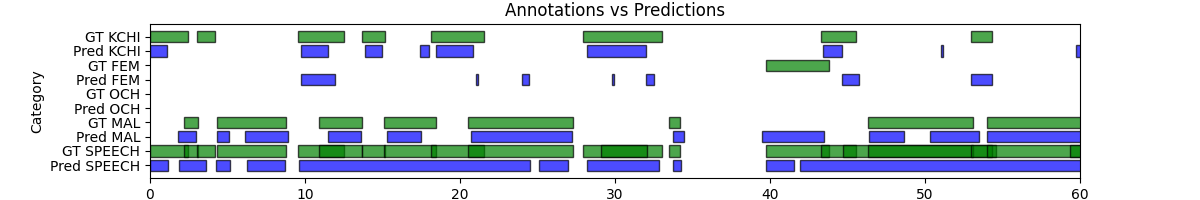
\includegraphics[width=6.67in]{images/vtc_performance_evaluation} 

}

\caption{VTC Predictions compared to Ground Truth Annotations}\label{fig:vtc-evaluations}
\end{figure}

\section{General Discussion}\label{general-discussion}

We present the ChildLens dataset, a diverse egocentric video-audio dataset documenting children's everyday experiences with annotations for key activities. The dataset's quality is demonstrated by its ability to yield strong results when applied to previously well-performing models for activity localization and audio classification. For instance, the pretrained Voice-Type Classifier for audio transcription achieves performance comparable to previous datasets. Similarly, the Boundary-Matching Network, applied to the ChildLens data for activity localization, produces robust results consistent with its performance on other datasets. This highlights the dataset's robustness in supporting well-established models, validating its quality for further research in multimodal analysis, particularly in the context of children's everyday experiences.

By integrating both visual and auditory information, this egocentric multimodal data enables a deeper understanding of children's daily experiences. Research shows that multimodal analysis can enhance activity understanding, as seen in datasets like UESTC-MMEA-CL (Xu et al., 2023) and the Nymeria dataset (Ma et al., 2024). By merging video and audio modalities, our work underscores the potential to better understand the context of children's interactions and behaviors, offering a clearer picture of their cognitive, emotional, and social development. For instance, enhancing activity localization with object identification could allow for tracking the objects children interact with during daily routines, as explored in multimodal adult-focused studies (Kazakos, Huh, Nagrani, Zisserman, \& Damen, 2021). Additionally, research by Bambach et al. (Bambach, Lee, Crandall, \& Yu, 2015) underscores the importance of hand detection in egocentric video for activity recognition. Their method, using Convolutional Neural Networks for precise hand segmentation, demonstrates how tracking hands can help distinguish between activities. This approach highlights the potential for hand tracking to enrich our understanding of children's interactions and behavior.

One limitation of our dataset is the class imbalance, with some activity classes underrepresented, which can affect model training and evaluation. Techniques like resampling, class merging, or augmentation could mitigate this issue and improve performance (Alani, Cosma, \& Taherkhani, 2020; Spelmen \& Porkodi, 2018). Additionally, selection bias may arise due to parents' control over when and how often they record activities, leading to variability in the data. The dataset's focus on families from a mid-sized German city further limits its diversity. Expanding the dataset to include broader cultural and geographic and backgrounds would enhance its generalizability. Addressing these challenges will improve the dataset's quality and make the conclusions drawn from it more robust, enhancing its potential for use in a wider range of contexts in multimodal child development research.

Finally, it is worth noting the unique contribution of this dataset, as most multimodal egocentric research focuses on adult perspectives (Núñez-Marcos, Azkune, \& Arganda-Carreras, 2022). Applying and adapting these methods to children's perspectives, as demonstrated by the ChildLens dataset, offers a valuable opportunity to extend existing research. This work underscores the need to develop specialized tools and methodologies for analyzing children's egocentric data to advance our understanding of children's cognitive, emotional, and social growth in diverse and meaningful ways.
\newpage
\# References

\begingroup
\setlength{\parindent}{-0.5in}
\setlength{\leftskip}{0.5in}

\phantomsection\label{refs}
\begin{CSLReferences}{1}{0}
\bibitem[\citeproctext]{ref-alaniClassifyingImbalancedMultimodal2020}
Alani, A. A., Cosma, G., \& Taherkhani, A. (2020). Classifying {Imbalanced Multi-modal Sensor Data} for {Human Activity Recognition} in a {Smart Home} using {Deep Learning}. \emph{2020 {International Joint Conference} on {Neural Networks} ({IJCNN})}, 1--8. Glasgow, United Kingdom: IEEE. \url{https://doi.org/10.1109/IJCNN48605.2020.9207697}

\bibitem[\citeproctext]{ref-bambachLendingHandDetecting2015}
Bambach, S., Lee, S., Crandall, D. J., \& Yu, C. (2015). Lending {A Hand}: {Detecting Hands} and {Recognizing Activities} in {Complex Egocentric Interactions}. \emph{2015 {IEEE International Conference} on {Computer Vision} ({ICCV})}, 1949--1957. Santiago, Chile: IEEE. \url{https://doi.org/10.1109/ICCV.2015.226}

\bibitem[\citeproctext]{ref-borjonViewTheirOwn2018}
Borjon, J. I., Schroer, S. E., Bambach, S., Slone, L. K., Abney, D. H., Crandall, D. J., \& Smith, L. B. (2018). A {View} of {Their Own}: {Capturing} the {Egocentric View} of {Infants} and {Toddlers} with {Head-Mounted Cameras}. \emph{Journal of Visualized Experiments}, (140), 58445. \url{https://doi.org/10.3791/58445-v}

\bibitem[\citeproctext]{ref-mmaction2contributorsOpenMMLabsNextGeneration2020}
Contributors, M. (2020). \emph{{OpenMMLab}'s {Next Generation Video Understanding Toolbox} and {Benchmark}}. Retrieved from \url{urlhttps://github.com/open-mmlab/mmaction2}

\bibitem[\citeproctext]{ref-debarbaroTenLessonsInfants2022}
De Barbaro, K., \& Fausey, C. M. (2022). Ten {Lessons About Infants}' {Everyday Experiences}. \emph{Current Directions in Psychological Science}, \emph{31}(1), 28--33. \url{https://doi.org/10.1177/09637214211059536}

\bibitem[\citeproctext]{ref-kapidisObjectDetectionBasedLocation2020}
Kapidis, G., Poppe, R., Van Dam, E., Noldus, L. P. J. J., \& Veltkamp, R. C. (2020). Object {Detection-Based Location} and {Activity Classification} from {Egocentric Videos}: {A Systematic Analysis}. In F. Chen, R. I. García-Betances, L. Chen, M. F. Cabrera-Umpiérrez, \& C. Nugent (Eds.), \emph{Smart {Assisted Living}} (pp. 119--145). Cham: Springer International Publishing. \url{https://doi.org/10.1007/978-3-030-25590-9_6}

\bibitem[\citeproctext]{ref-kazakosLittleHelpMy2021}
Kazakos, E., Huh, J., Nagrani, A., Zisserman, A., \& Damen, D. (2021). With a {Little Help} from my {Temporal Context}: {Multimodal Egocentric Action Recognition}. \url{https://doi.org/10.48550/ARXIV.2111.01024}

\bibitem[\citeproctext]{ref-lavechinOpensourceVoiceType2020}
Lavechin, M., Bousbib, R., Bredin, H., Dupoux, E., \& Cristia, A. (2020). An open-source voice type classifier for child-centered daylong recordings. \url{https://doi.org/10.48550/ARXIV.2005.12656}

\bibitem[\citeproctext]{ref-linBMNBoundaryMatchingNetwork2019}
Lin, T., Liu, X., Li, X., Ding, E., \& Wen, S. (2019). {BMN}: {Boundary-Matching Network} for {Temporal Action Proposal Generation}. \url{https://doi.org/10.48550/ARXIV.1907.09702}

\bibitem[\citeproctext]{ref-longBabyViewDatasetHighresolution2024}
Long, B., Xiang, V., Stojanov, S., Sparks, R. Z., Yin, Z., Keene, G. E., \ldots{} Frank, M. C. (2024, June 14). The {BabyView} dataset: {High-resolution} egocentric videos of infants' and young children's everyday experiences. \url{https://doi.org/10.48550/arXiv.2406.10447}

\bibitem[\citeproctext]{ref-maNymeriaMassiveCollection2024}
Ma, L., Ye, Y., Hong, F., Guzov, V., Jiang, Y., Postyeni, R., \ldots{} Newcombe, R. (2024). Nymeria: {A Massive Collection} of {Multimodal Egocentric Daily Motion} in the {Wild}. \url{https://doi.org/10.48550/ARXIV.2406.09905}

\bibitem[\citeproctext]{ref-nunez-marcosEgocentricVisionbasedAction2022}
Núñez-Marcos, A., Azkune, G., \& Arganda-Carreras, I. (2022). Egocentric {Vision-based Action Recognition}: {A} survey. \emph{Neurocomputing}, \emph{472}, 175--197. \url{https://doi.org/10.1016/j.neucom.2021.11.081}

\bibitem[\citeproctext]{ref-rogoffImportanceUnderstandingChildrens2018}
Rogoff, B., Dahl, A., \& Callanan, M. (2018). The importance of understanding children's lived experience. \emph{Developmental Review}, \emph{50}, 5--15. \url{https://doi.org/10.1016/j.dr.2018.05.006}

\bibitem[\citeproctext]{ref-royPredictingBirthSpoken2015}
Roy, B. C., Frank, M. C., DeCamp, P., Miller, M., \& Roy, D. (2015). Predicting the birth of a spoken word. \emph{Proceedings of the National Academy of Sciences}, \emph{112}(41), 12663--12668. \url{https://doi.org/10.1073/pnas.1419773112}

\bibitem[\citeproctext]{ref-saberCurriculumLearningInfant2023}
Saber, S., Hansaria, H., Wood, J. N., Smith, L. B., \& Tiganj, Z. (2023). Curriculum learning with infant egocentric videos. \emph{NIPS '23: Proceedings of the 37th International Conference on Neural Information Processing Systems}, 54199--54212.

\bibitem[\citeproctext]{ref-smithContributionsHeadMountedCameras2015}
Smith, L. B., Yu, C., Yoshida, H., \& Fausey, C. M. (2015). Contributions of {Head-Mounted Cameras} to {Studying} the {Visual Environments} of {Infants} and {Young Children}. \emph{Journal of Cognition and Development}, \emph{16}(3), 407--419. \url{https://doi.org/10.1080/15248372.2014.933430}

\bibitem[\citeproctext]{ref-spanglerToddlersEverydayExperiences1989}
Spangler, G. (1989). Toddlers' {Everyday Experiences} as {Related} to {Preceding Mental} and {Emotional Disposition} and {Their Relationship} to {Subsequent Mental} and {Motivational Development}: {A Short-Term Longitudinal Study}. \emph{International Journal of Behavioral Development}, \emph{12}(3), 285--303. \url{https://doi.org/10.1177/016502548901200301}

\bibitem[\citeproctext]{ref-spelmenReviewHandlingImbalanced2018}
Spelmen, V. S., \& Porkodi, R. (2018). A {Review} on {Handling Imbalanced Data}. \emph{2018 {International Conference} on {Current Trends} Towards {Converging Technologies} ({ICCTCT})}, 1--11. Coimbatore: IEEE. \url{https://doi.org/10.1109/ICCTCT.2018.8551020}

\bibitem[\citeproctext]{ref-sullivanSAYCamLargeLongitudinal2021}
Sullivan, J., Mei, M., Perfors, A., Wojcik, E., \& Frank, M. C. (2021). {SAYCam}: {A Large}, {Longitudinal Audiovisual Dataset Recorded From} the {Infant}'s {Perspective}. \emph{Open Mind}, \emph{5}, 20--29. \url{https://doi.org/10.1162/opmi_a_00039}

\bibitem[\citeproctext]{ref-truongCrossviewActionRecognition2024}
Truong, T.-D., \& Luu, K. (2024). Cross-view action recognition understanding from exocentric to egocentric perspective. \emph{Neurocomputing}, 128731. \url{https://doi.org/10.1016/j.neucom.2024.128731}

\bibitem[\citeproctext]{ref-tsutsuiComputationalModelEarly2020}
Tsutsui, S., Chandrasekaran, A., Reza, M. A., Crandall, D., \& Yu, C. (2020, June 4). A {Computational Model} of {Early Word Learning} from the {Infant}'s {Point} of {View}. \url{https://doi.org/10.48550/arXiv.2006.02802}

\bibitem[\citeproctext]{ref-xuContinualEgocentricActivity2023}
Xu, L., Wu, Q., Pan, L., Meng, F., Li, H., He, C., \ldots{} Dai, Y. (2023). \emph{Towards {Continual Egocentric Activity Recognition}: {A Multi-modal Egocentric Activity Dataset} for {Continual Learning}}. \url{https://doi.org/10.48550/ARXIV.2301.10931}

\bibitem[\citeproctext]{ref-yoshidaWhatsViewToddlers2008}
Yoshida, H., \& Smith, L. B. (2008). What's in {View} for {Toddlers}? {Using} a {Head Camera} to {Study Visual Experience}. \emph{Infancy}, \emph{13}(3), 229--248. \url{https://doi.org/10.1080/15250000802004437}

\end{CSLReferences}

\endgroup

\newpage

\section{Appendix}\label{appendix}

\subsection{List of ChildLens Activity Classes}\label{list-of-childlens-activity-classes}

The dataset contains the following list of activities.

\begin{enumerate}
\def\labelenumi{\arabic{enumi}.}
\tightlist
\item
  \textbf{playing with object}: The child is playing with an object, such as a toy or a ball.
\item
  \textbf{playing without object}: The child is playing without an object, such as playing hide and seek or catch.
\item
  \textbf{pretend play}: The child is engaged in imaginative play, such as pretending to be a doctor or a firefighter.
\item
  \textbf{watching something}: The child is watching a movie, TV show, or video on either a screen or a device.
\item
  \textbf{reading book}: The child is reading a book or looking at pictures in a book.
\item
  \textbf{child talking}: The child is talking to themselves or to someone else.
\item
  \textbf{other person talking}: Another person is talking to the child.
\item
  \textbf{overheard speech}: Conversations that the child can hear but is not directly involved in.
\item
  \textbf{drawing}: The child is drawing or coloring a picture.
\item
  \textbf{crafting things}: The child is engaged in a craft activity, such as making a bracelet or decoration.
\item
  \textbf{singing / humming}: The child is singing or humming a song or a melody.
\item
  \textbf{making music}: The child is playing a musical instrument or making music in another way.
\item
  \textbf{dancing}: The child is dancing to music or moving to a rhythm.
\item
  \textbf{listening to music / audiobook}: The child is listening to music or an audiobook.
\end{enumerate}

\subsection{List of ChildLens Location Classes}\label{list-of-childlens-location-classes}

\begin{enumerate}
\def\labelenumi{\arabic{enumi}.}
\tightlist
\item
  livingroom
\item
  playroom
\item
  bathroom
\item
  hallawy
\item
  other
\end{enumerate}

\subsection{Activity Class Statistics}\label{activity-class-statistics}

\begin{table}[tbp]

\begin{center}
\begin{threeparttable}

\caption{\label{tab:activity-classes-statistics}Number of video instances and the total duration (in minutes).}

\begin{tabular}{llll}
\toprule
Category & \multicolumn{1}{c}{Activity Class} & \multicolumn{1}{c}{Instance Count} & \multicolumn{1}{c}{Total Duration (min)}\\
\midrule
Audio & Child talking & 100 & 100\\
 & Other person talking & 100 & 100\\
 & Overheard Speech & 100 & 100\\
 & Singing/Humming & 100 & 100\\
 & Listening to music/audiobook & 100 & 100\\
Video & Watching something & 2 & 5.09\\
 & Drawing & 62 & 374.91\\
 & Crafting things & 26 & 109.14\\
 & Dancing & 2 & 0.57\\
Multimodal & Playing with object & 318 & 1371.08\\
 & Playing without object & 25 & 28.87\\
 & Pretend play & 59 & 158.84\\
 & Reading a book & 83 & 334.19\\
 & Making music & 3 & 2.13\\
\bottomrule
\end{tabular}

\end{threeparttable}
\end{center}

\end{table}


\end{document}
